GPU会在下一个例子中进行展示,不过对于任何类型的加速器都一样。为了针对常见的加速器类,设备分为几个大类,SYCL提供了内置的选择器类。要从设备类型类别中进行选择,例如“系统中可用的GPU”,相应的代码非常短。\par

\hspace*{\fill} \par %插入空行
\textbf{设备类型}

队列可以绑定的设备主要有两类:\par

\begin{enumerate}
	\item 主机。
	\item 加速设备,如GPU、FPGA或CPU设备,用于加速程序中的负载。
\end{enumerate}

\hspace*{\fill} \par %插入空行
\textbf{加速器设备}

加速器类型主要有以下几种:\par

\begin{enumerate}
	\item CPU设备
	\item GPU设备
	\item 加速器,捕捉既不为CPU,也不是GPU的设备。这包括FPGA和DSP。
\end{enumerate}

使用内置的选择器类,这些类别中的任何设备都可以很容易地绑定到队列,这些选择器类可以传递到队列(和其他一些类)的构造中。\par

\hspace*{\fill} \par %插入空行
\textbf{设备选择器}

必须绑定到特定设备的类,如:queue类。其构造函数可以接受从device\_selector派生的类。queue构造函数是\par

\begin{tcolorbox}[colback=green!5!white,colframe=green!75!black]
queue( const device\_selector \&deviceSelector, const property\_list \&propList = \{\});
\end{tcolorbox}

有5种常用的内置选择器:\par

\hspace*{\fill} \par %插入空行
\begin{tabular}{lp{10cm}p{10cm}}
	\toprule  %添加表格头部粗线
	\textbf{default\_selector}& 默认选择设备 \\
	\textbf{host\_selector}& 选择主机(始终可用) \\
	\textbf{cpu\_selector}& 选择一个标识为CPU的设备\\
	\textbf{gpu\_selector}& 选择一个标识为GPU的设备\\
	\textbf{accelerator\_selector}&选择一个标识为“加速器”的设备,其中包括FPGA。\\
	\bottomrule %添加表格底部粗线
\end{tabular}

\hspace*{\fill} \par %插入空行
DPC++中包含的另一个选择器(SYCL中不可用)可以通过包含头文件\\
"CL/sycl/intel/fpga\_extensions.hpp"来使用:

\hspace*{\fill} \par %插入空行
\begin{tabular}{lp{10cm}p{10cm}}
	\toprule  %添加表格头部粗线
	\textbf{INTEL::fpga\_selector} & 选择一个标识为FPGA的设备\\
	\bottomrule %添加表格底部粗线
\end{tabular}

\hspace*{\fill} \par %插入空行
可以使用内置选择器来构造队列,例如:\par

\begin{tcolorbox}[colback=green!5!white,colframe=green!75!black]
queue myQueue\{ cpu\_selector\{\} \};
\end{tcolorbox}

图2-10给出了使用cpu\_selector的完整示例,图2-11给出了队列与可用CPU设备的对应绑定。\par

图2-12展示了使用各种内置选择器类的例子,演示了设备选择器与另一个类(device)的使用,该类在构造时接受一个device\_selector。\par

\hspace*{\fill} \par %插入空行
图2-10 CPU设备选择器示例
\begin{lstlisting}[caption={}]
#include <CL/sycl.hpp>
#include <iostream>
using namespace sycl;

int main() {
	// Create queue to use the CPU device explicitly
	queue Q{ cpu_selector{} };
	
	std::cout << "Selected device: " <<
		Q.get_device().get_info<info::device::name>() << "\n";
	std::cout << " -> Device vendor: " <<
		Q.get_device().get_info<info::device::vendor>() << "\n";
		
	return 0;
}
// Possible Output:
// Selected device: Intel(R) Core(TM) i5-7400 CPU @ 3.00GHz
//  -> Device vendor: Intel(R) Corporation
\end{lstlisting}

\hspace*{\fill} \par %插入空行
图2-11 将CPU设备绑定到程序队列
\begin{center}
	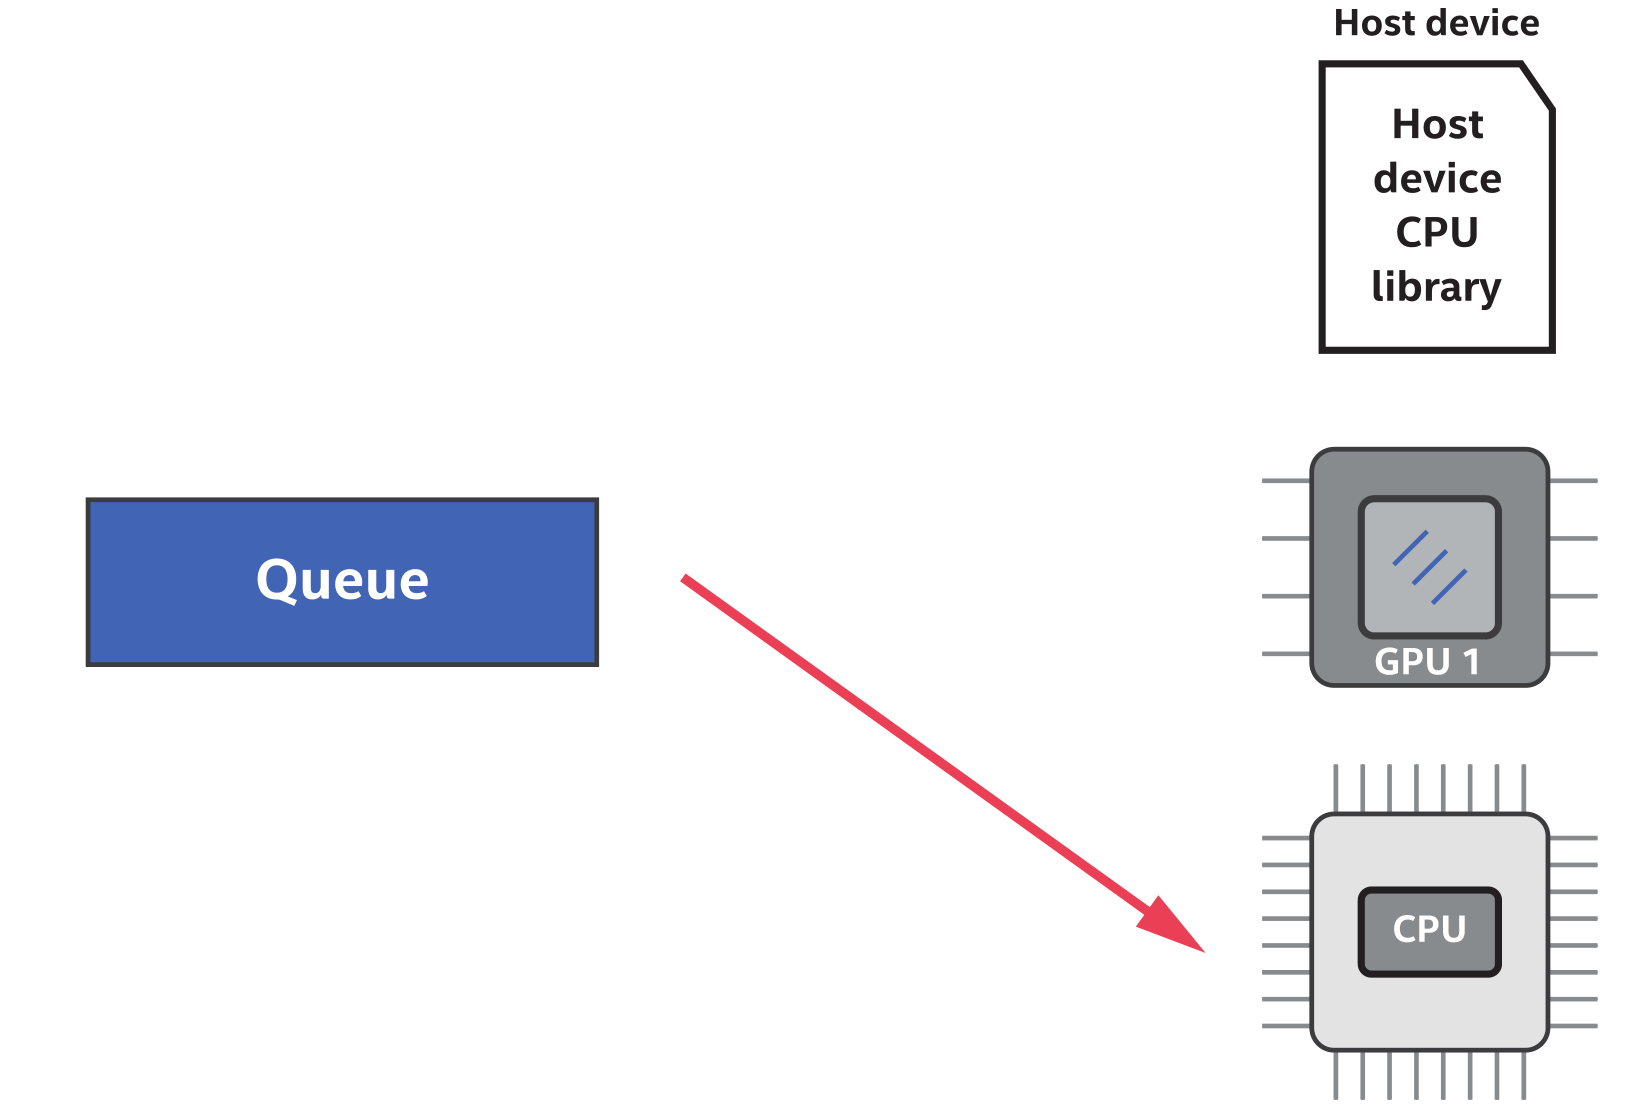
\includegraphics[width=0.7\textwidth]{content/chapter-2/images/7}
\end{center}

\hspace*{\fill} \par %插入空行
图2-12 各种设备选择器类的标识输出,设备选择器可以用于构造多个队列(本例中,构造了类实例)
\begin{lstlisting}[caption={}]
#include <CL/sycl.hpp>
#include <CL/sycl/INTEL/fpga_extensions.hpp> // For fpga_selector
#include <iostream>
#include <string>
using namespace sycl;

void output_dev_info( const device& dev, 
					  const std::string& selector_name) {
	std::cout << selector_name << ": Selected device: " <<
		dev.get_info<info::device::name>() << "\n";
	std::cout << " -> Device vendor: " <<
		dev.get_info<info::device::vendor>() << "\n";
}

int main() {
	output_dev_info( device{ default_selector{}}, 
							"default_selector" );
	output_dev_info( device{ host_selector{}}, 
							"host_selector" );
	output_dev_info( device{ cpu_selector{}}, 
							"cpu_selector" );
	output_dev_info( device{ gpu_selector{}}, 
							"gpu_selector" );
	output_dev_info( device{ accelerator_selector{}},
							"accelerator_selector" );
	output_dev_info( device{ INTEL::fpga_selector{}}, 
							"fpga_selector" );
	
	return 0;
}

//Possible Output:
//default_selector: Selected device: Intel(R) Gen9 HD Graphics NEO
//					-> Device vendor: Intel(R) Corporation
//host_selector: Selected device: SYCL host device
//					-> Device vendor:
//cpu_selector: Selected device: Intel(R) Core(TM) i5-7400 CPU @ 3.00GHz
//					-> Device vendor: Intel(R) Corporation
//gpu_selector: Selected device: Intel(R) Gen9 HD Graphics NEO
//					-> Device vendor: Intel(R) Corporation
//accelerator_selector: Selected device: Intel(R) FPGA Emulation Device
//					-> Device vendor: Intel(R) Corporation
//fpga_selector: Selected device: pac_a10 : PAC Arria 10 Platform
//					-> Device vendor: Intel Corp
\end{lstlisting}

\hspace*{\fill} \par %插入空行
\textbf{设备选择失败时}

gpu\_selector创建的对象(比如:队列)使用时,但没有可供运行时使用的GPU设备,那么这个选择器会抛出runtime\_error异常。对于所有的设备选择器类都是如此,没有所需的设备可用,则抛出runtime\_error异常。对于复杂的应用程序来说,捕获这个错误并使用不太理想的(对于应用程序/算法)设备类作为替代是合理的。异常和错误处理将在第5章中详细讨论。\par





